\section{Actividad No 03 –  Creating PL/SQL Blocks} 
		
\begin{enumerate}[1.]
	\item VOCABULARIO :
	\subitem Identify the vocabulary word for each definition below:
	\subitem 01-\_\_\_\_\_\_\_\_\_\_\_\_\_\_\_\_:Unnamed blocks of code not stored in the database and do not exist after they are executed
	\subitem 02-\_\_\_\_\_\_\_\_\_\_\_\_\_\_\_\_:A program that computes and returns a single value
	\subitem 03-\_\_\_\_\_\_\_\_\_\_\_\_\_\_\_\_:Named PL/SQL blocks that are stored in the database and can be declared as procedures or functions
	\subitem 04-\_\_\_\_\_\_\_\_\_\_\_\_\_\_\_\_:Software that checks and translates programs written in highlevel programming languages into binary code to execute
	\subitem 05-\_\_\_\_\_\_\_\_\_\_\_\_\_\_\_\_:A program that performs an action, but does not have to return a value
	\\\\
	\\01.- CHARACTERISTICS OF ANONYMOUS BLOCKS
	\\02.- FUNCTION
	\\03.- SUBPROGRAMS
	\\04.- C, JAVA, OL/SQL
	\\05.- PROCEDURE

	\item Try It / Solve It
	\subitem 01- Complete the following chart defining the syntactical requirements for a PL/SQL block:
	\begin{center}
	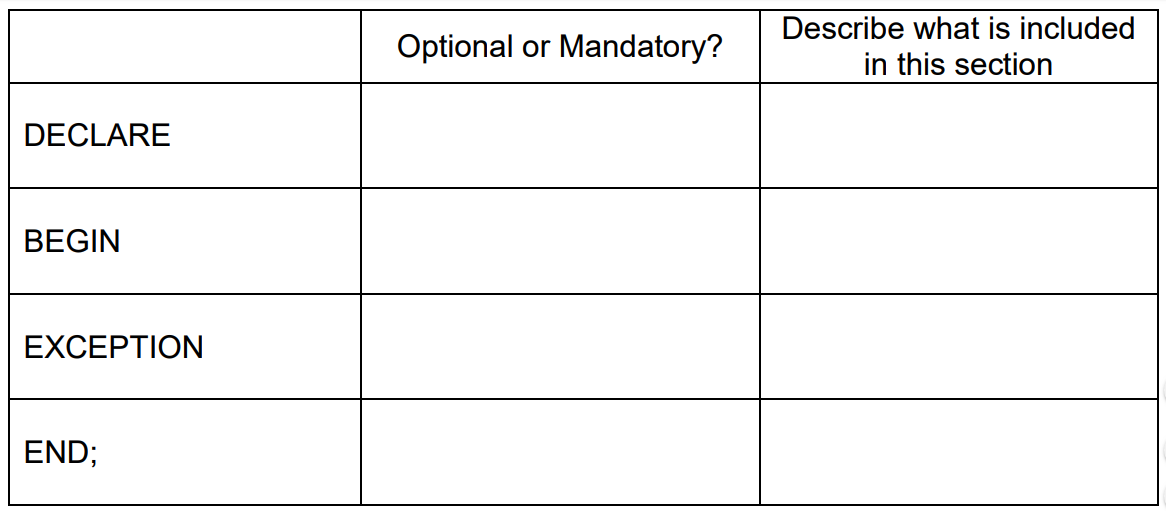
\includegraphics[width=15cm]{./Imagenes/actividad01}  
	\end{center}	

	   01.- DECLARE	= is optional -- 
	\\02.- BEGIN		= is Mandatory --
	\\03.- EXCEPTION	= is optional --
	\\04.- END		= is Mandatory --\\

	\subitem 02- Which of the following PL/SQL blocks executes successfully? For the blocks that fail, explain why they fail
	\\
	\subitem A. BEGIN
	\subitem    END;
	\subitem B. DECLARE
 	\subitem    amount INTEGER(10);
	\subitem    END;
	\subitem C. DECLARE
	 \subitem   BEGIN
	 \subitem   END;
	\subitem D. DECLARE
	 \subitem	amount NUMBER(10);
	 \subitem	begin
	 \subitem	DBMS\_OUTPUT.PUT\_LINE(amount);
	 \subitem	END;
	\\\\A.- ERROR ---------- FALTA EL EJECUTABLE
	\\B.-
	\\C.-
	\\D.- CORRECTO\\

	\subitem 03- Fill in the blanks:
	\subitem A. PL/SQL blocks that have no names are called \_\_\_\_\_\_\_\_\_\_\_\_\_\_\_\_\_\_.
	\subitem B. \_\_\_\_\_\_\_\_\_\_\_\_\_\_\_ and \_\_\_\_\_\_\_\_\_\_\_\_\_\_\_ are named blocks and are stored in the database.
	\\\\A.- ANONYMOUS BLOCKS
	\\B.- PROCEDURES --- FUNCTION

\end{enumerate}

